\documentclass[english]{article}
\usepackage[T1]{fontenc}
\usepackage[utf8]{inputenc}
\usepackage{geometry}
\geometry{verbose,tmargin=3.5cm,bmargin=4cm,lmargin=3.8cm,rmargin=3.8cm}

% plots
\usepackage{graphicx}
\graphicspath{ {../plots/} }

% newlines instead of indent for paragraphs
\usepackage[parfill]{parskip}
% tables
\usepackage{multirow}

% import natbib and sets bibliography and citation styles
\usepackage[numbers,sort]{natbib}
\bibliographystyle{apalike}

\makeatletter
\usepackage{hyperref}

\makeatother
\usepackage{babel}

% work in progress packages
\newcommand{\citationneeded}{\textsuperscript{\color{blue} [citation needed]}}
\usepackage{easy-todo}

\begin{document}

\listoftodos

\title{New Generation Iterative Prisoner’s Dilemma:\\ Keep your enemies closer and be loud about it}
\author{Martin Toman}
\date{06 May 2021}
\maketitle


\begin{abstract}
% The abstract should be short and give the overall idea:
% what is the background, the research questions, what is contribution, and what are the main conclusions.
% It should be readable as a stand-alone text (preferably no references to the paper or outside literature).

\todo{write abstract}
\end{abstract}


\section{Introduction}

% intro - what is prisoner's dilemma
How can we encourage and sustain cooperation? Humans dominate their environments thanks to our ability to cooperate flexibly and at scale, as argued by \citet{harari-sapiens}.
To study the conditions necessary for cooperation to flourish we need a suitable model of an activity with temptations to defect and punishments for doing so.

In 1950, Albert Tucker named a particular two-player exchange game "The Prisoner's Dilemma" \citep{sep-prisoner-dilemma}.
This game elegantly captures the difficulty of the decision between cooperation and defection in a single choice.
Despite being so simple compared to the complexity of the problem it is representing, it was used to model many aspects of behaviour in systems of selfish individuals; and, according to \citet{Axelrod84}, for "discovery of the precise conditions that are necessary and sufficient for cooperation to emerge".

% iterated version + the dilemma
In the case of a one-off exchange, there being no opportunity for a follow-up punishment, the rational behaviour is defection. (This extends to all rounds for a fixed-length game, inductively \citep{Axelrod84}.)
The interesting behaviour arises if there is no end; or, at least, if there is no way for the participants of the game to know when the game ends or even if there is an end.
% reputation importance
One has to expect that even a single defection can be infinitely punished by never again cooperating with the culprit \citep{GRIM}.
Such a risk may just not be worth it.

% global reputation system
The defectors can, naturally, only be punished if they can be identified and known to others. This is why services like Ebay or Airbnb have a rating system in place.
Presence of a reputation system has been shown to strongly boost cooperation, as shown by \citet{simple-reputation} and \citet{public-private-monitoring}.
These studies used groups of volunteers as game participants and explored the effects of various information being public - from only the latest move of the current opponent, to full histories of all moves taken by every participant.

% decentralizing reputation: keeping track internally?
These studies were limited by their use of humans as game participants and were thus limited to relatively small groups with few rounds; they also used external infrastructure for information passing: therefore eliminating noise, delays, and deliberately wrong information.
As shown by \citet{noise}, not all strategies that perform well in noise-less environments can do so under the presence of noise.

Using external infrastructure for passing information also meant that the transmission speed was uniform for all participants receiving all necessary information in time for their next round of the game.
These are non-trivial idealizations: relaxing them would yield a model closer to real-world systems and could change the results drastically.

In this paper we explore the feasibility of such a solution; we look at how well a local reputation system sustains cooperation and under what conditions does it yield optimal results.
We evaluate the approach under varying gossip range and memory length; and conclude the effectiveness of local reputation in enforcing cooperation in spatial prisoner's dilemma.

\todo{outline the structure of the paper}


\section{Methodology or Problem Description}
\todo{add section introduction}

\subsection{Methodology}
% Typically in general research articles, the second section contains a description of the research methodology, explaining what you, the researcher, is doing to answer the research question(s), and why you have chosen this method.
% For purely analytical work this is a description of the data collection or experimental setup on how to test the hypothesis, with a motivation.
% In any case this section includes references to necessary background information.

To explore the effects of local reputation, built via openly gossiping with local peers, we are gonna use a computer simulation of a multi-agent spatial environment; we will base it on the design of Spatial Iterated Prisoner’s Dilemma, as used by \citet{smaldino}.
A single round of the game is defined using a payoff matrix as shown in Table \ref{table:payoff}, with $T > R > P > S$ and $2R > T + S$ \citep{chammah1965}.

\begin{table}[h!]
  \centering
  \begin{tabular}{c c||c|c}
    & & \multicolumn{2}{c}{Opponent's move} \\
    & & Cooperate & Defect \\
    \hline\hline

    \multirow{4}{6em}{Player's move}
    & \multirow{2}{5em}{Cooperate}
      & Player:\ \ \ \ \ \ R & Player:\ \ \ \ \ \ S \\
    & & Opponent: R & Opponent: T \\
    \cline{2-4}
    & \multirow{2}{5em}{Defect}
      & Player:\ \ \ \ \ \ T & Player:\ \ \ \ \ \ P \\
    & & Opponent: S & Opponent: P \\
  \end{tabular}

  \caption{Payoff matrix}
  \label{table:payoff}
\end{table}

Participants are agents living in a 2D grid, accumulating energy via repeatably engaging in rounds of PD as defined above. Agents are moving at the same speed, and their order in which they take their turn is randomly determined at every clock tick. They pay a fixed cost to survive to a next round, which is subtracted from all peers at the end of each turn (agents who deplete their energy die and are removed from the simulation).
Another use of the energy is to constrain reproduction and allow only the most successful agents to reproduce, producing an offspring with an identical strategy.

We will expand the model by giving the agents a (limited) memory to keep track of past actions of other participants and later allow them to actively and freely share this knowledge by gossiping at various range.

To determine the effectives of gossiping in inducing cooperation, we will observe the rate of convergence to a population of cooperators, stopping the game once stable equilibrium is achieved. We will use the no-gossip model as a benchmark and compare various range at which gossiping is possible to determine the optimal amount of information transmitted necessary for cooperation to win in the population.
After that we will compress the gossip into only labels ("hostile"/"neutral"/"friendly") determined by agents based on their local observations.





% \subsection{Formal Problem Description}
% For some types of work in computer science the methodology is standard: analyze the problem (e.g., make assumptions and derive properties), present a new algorithm and its theoretical background, proving its correctness, and evaluate unproven aspects in simulation.
% Then an explanation of the methodology is often omitted, and the setup of the evaluation is part of a later section on the evaluation of the ideas.\footnote{This already shows that there is no single outline to be given for all papers.}
% In this case, explain relevant concepts, theory and models in this section (with references) and relate them to your research question.
% Also this section then typically contains a more precise, formal description of the problem.

% Do not forget to give this section another name, for example after the problem you are solving.

% \section{Your contribution}
% In computer science typically the third section contains an exposition of the main ideas, for example the development of a theory, the analysis of the problem (some proofs), a new algorithm, and potentially some theoretical analysis of the properties of the algorithm.

% Do not forget to give this section another name, for example after the method or idea you are presenting.

% Some more detailed suggestions for typical types of contributions in computer science are described in the following subsections.

% \subsection*{Experimental work}
% In this case, this section will mostly contain a description of the methods/algorithms you will be comparing. Although not all methods need to be described in detail (providing appropriate references are available), make sure that you reveal sufficient details to a reader not familiar with these methods to: a) obtain a high-level understanding of the method and differences between them, and b) understand your explanation of the results.

% \subsection*{Improvement of an idea}
% In this case, you would need to explain in detail how the improvement works. If it is based on some observation that can be proven, this is a good place to provide that proof (e.g., of the correctness of your approach).

\section{Experimental Setup and Results}
% As discussed earlier, in many sciences the methodology is explained in section 2 and this section only discusses the results.
% However, in computer science, most often the details of the evaluation setup are described here first (simulation environment, etc.).
% Very important here is that any skilled reader would be able to reproduce this setup and then obtain the same results.

% Then, results are reported in an accessible manner through figures (preferably with captions that allow them to be understood without going through the whole text), observations are made that clearly follow from the presented results.
% Conclusions are drawn that follow logically from the previous material.
% Sometimes the conclusions are in fact hypotheses, which in turn may give rise to new experiments to be validated.

\begin{figure}[h!]
  \centering
  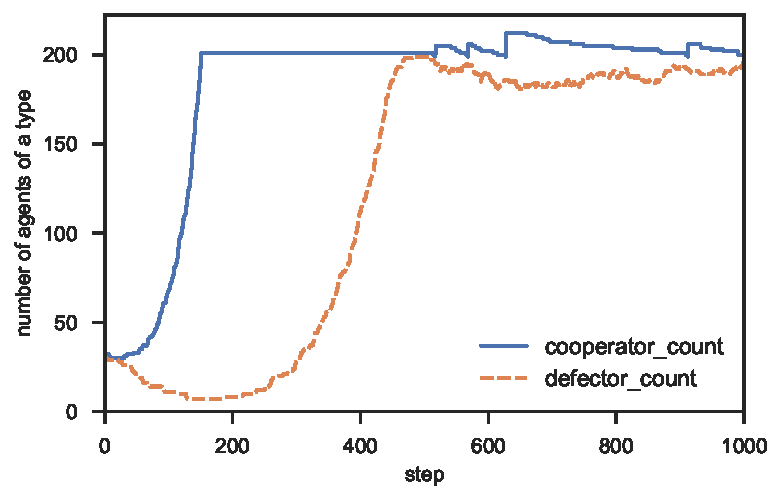
\includegraphics{frequency_time_with_memory.pdf}
  \caption{Evolution of agent population over time (memory size = 1)}
  \label{table:population_evolution}
\end{figure}

\begin{figure}[h!]
  \centering
  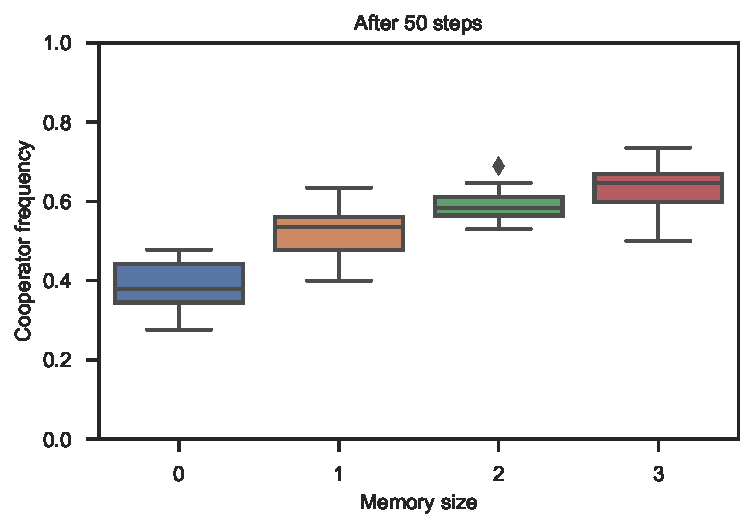
\includegraphics{cooperator_frequency_memory_50steps.pdf}
  \caption{Agent type frequency after $50$ steps}
  \label{table:cooperator_frequency_converged_50}
\end{figure}
\begin{figure}[h!]
  \centering
  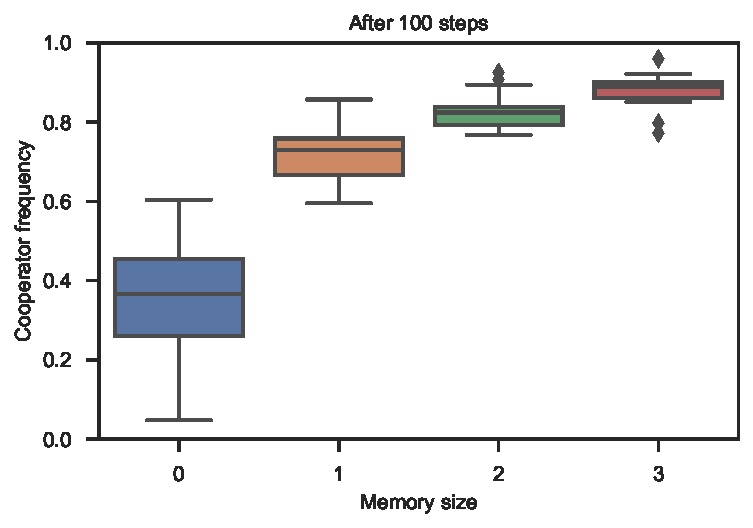
\includegraphics{cooperator_frequency_memory_100steps.pdf}
  \caption{Agent type frequency after $100$ steps}
  \label{table:cooperator_frequency_converged_100}
\end{figure}

% You may want to give this section another name.
\todo{name this section}



\section{Responsible Research}
% Reflect on the ethical aspects of your research and discuss the reproducibility of your methods.

% \section{Discussion}
% Results can be compared to known results and placed in a broader context.
% Provide a reflection on what has been concluded and how this was done.
% Then give a further possible explanation of results.

% You may give this section another name, or merge it with the one before or the one hereafter.



\section{Conclusions and Future Work}
% Summarize the research question(s) and the answers to the research question(s).
% Make statements.
% Highlight interesting elements.

% Discuss open issues, possible improvements, and new questions that arise from this work; formulate recommendations for further research.

% ideally, this section can stand on its own: it should be readable without having read the earlier sections.

\pagebreak
\bibliography{references}

\end{document}
